\xchapter{基于超宽带虚拟阵列的物体三维点云重建}{3D Object Point Cloud Reconstruction Based on Ultra-Wideband Virtual Array}
\xsection{引言}{Introduction}
物体三维重建一直作为一个重要的研究领域，其目的在于利用各种类型的输入来恢复出物体的三维结构，例如点云、网格和体素等。然而，目前的物体三维重建领域的主流研究方向是基于二维RGB图像的三维重建，该类方法的缺陷在于极其依赖场景的可见性和光照条件，在存在遮挡和光照环境恶劣的情况下，该类方法将不再适用。也有部分研究人员使用射频传感器来进行物体三维重建，这类方法不依赖于环境光照，并且由于射频的穿透能力可以有效地解决遮挡问题，但其中大部分方法依赖于集成了多根发射天线和多根接收天线的复杂且昂贵的射频设备，并且大部分工作聚焦于恢复人体这一较为简单固定的形状模式，对于普适的物体形状并不适用。

本章将介绍本文的第一个主要贡献点，即提出了一种基于超宽带虚拟阵列的物体三维点云重建方法，该方法?
\xsection{超宽带虚拟阵列信号采集与处理}{Ultra-Wideband Virtual Array Signal Acquisition and Processing}
\xsubsection{超宽带虚拟阵列构建}{Ultra-Wideband Virtual Array Construction}
使用仅具有单根发射天线和单根接收天线的超宽带雷达去进行物体三维重建是极具挑战性的，原因在于：（1）超宽带雷达使用的射频信号波长较大，因此感知分辨率相较于RGB相机甚至是毫米波雷达都远远不足；（2）大多数雷达系统为了提升雷达感知能力，通常会集成多根发射天线（$T$根）和多根接收天线（$R$根）去等效出$T\times R$根虚拟天线来提升雷达分辨率，而单发单收的超宽带雷达不具备这样的能力。因此，想要使用单发单收的超宽带雷达来进行物体的三维重建，必须要提升雷达的感知能力。

受到逆合成孔径雷达(Inverse Synthetic Aperture Radar,ISAR)的启发，本文通过使被重建物体相对于雷达运动起来，来生成大量的虚拟雷达天线，从而提升雷达的感知能力。首先介绍一下被人们熟知的合成孔径雷达(Synthetic Aperture Radar,SAR)，SAR是一种利用雷达平台的运动来合成更大孔径雷达天线的技术，SAR系统一般被安装在移动平台上例如飞机、卫星等，平台沿着预定路径移动，在移动过程中，雷达连续发射脉冲信号并接收回波信号，在每一个雷达发射脉冲信号的位置都可以等效出一个虚拟雷达天线，通过这种方式，可以模拟出一个大的虚拟天线孔径，大大提升雷达的感知分辨率。ISAR和SAR的原理相似，ISAR也是利用雷达和物体之间的相对运动来合成更大孔径雷达天线，不同之处在于ISAR是通过物体自身运动来产生这种相对运动，因此被称为逆合成孔径雷达。本文利用ISAR的原理，让物体相对于超宽带雷达运动起来，这种运动又可以等效为雷达相对于物体的运动，在雷达每一次发射超宽带脉冲信号的位置都可以等效出一个超宽带虚拟天线，物体的一次持续运动可以产生巨量的虚拟天线构成一个虚拟阵列，原理如图?所示。让物体相对雷达运动起来看似是一个比较严苛的条件，然而在物流、安检等场景下，物体是需要被放置在传送带上进行运输的，此时，我们只需将雷达系统安装在传送带侧边，就可以让物体相对于雷达产生稳定匀速的相对运动，本文提出的三维点云重建方法恰好也是针对物流、安检这些物体有可能被轻薄包装包裹的场景。

上面介绍了本文构建超宽带虚拟阵列的方法，下面我们重新探究构建虚拟阵列后雷达接收到二维矩阵信号的物理意义。在上一章中已经介绍过，一段连续时间内，超宽带雷达采集到的数据为一个二维复数矩阵，矩阵的慢时间轴代表着不同的采样帧，快时间轴代表着不同的距离箱。当雷达和物体相对运动时，由于每个帧的时间极短（数百微秒），帧内位移极小，因此我们可以认为在一个帧内，雷达和物体是相对静止的，进而可以认为，雷达在一个帧内不同快时间上的采样其实是一个虚拟天线在固定位置上对不同快时间的采样。因此，此时二维矩阵的慢时间维度意义发生改变，慢时间维度对应的是不同的虚拟超宽带天线。

综上所述，本文通过物体和雷达之间的相对运动来为雷达构建出大量的虚拟天线组成大型超宽带虚拟阵列，来大幅提升超宽带雷达的感知能力，超宽带雷达接收到的二维矩阵信号，慢时间轴对应的是不同的虚拟天线，快时间轴对应的是不同的距离箱。同时，由于仅从单一视角去用上述方法采集信号，我们很难获取到物体侧面及背面的几何结构信息，因此，我们会从物体的四个不同视角使用上述方法去进行信号的采集，最终，采集到的四个二维复数矩阵会送入后续的处理流程。
\xsubsection{背景反射消减}{Background Reflection Reduction}
由于超宽带雷达不仅会被目标物体所反射，也会被环境中的其他非目标物体所反射，雷达最终得到的接收信号里实际也包含了这部分信号，会对目标信号产生干扰，同时，由于发射天线和接收天线之间的串扰(Crosstalks)，即发射天线到接收天线之间的直接信号泄露，会导致每个接收帧的前几个距离箱的信号幅值异常强烈，如图?，这两种干扰会影响我们对目标信号的定位和后续处理产生影响，我们将这两种干扰信号统称为背景反射。为了避免背景反射对目标信号的影响，需要对这部分发射进行消减。

回顾第二章对接收信号的基础建模，我们可以将接收信号再进一步细化：
\begin{equation}
    \begin{aligned}
        y(t) &= \frac{1}{2}\sum_{p\_target=1}^{P\_target}\alpha_{p\_target}g(t-kT_S-T_{p\_target})\cdot e^{j\theta_{p\_target}} \\
            &+ \frac{1}{2}\sum_{p\_other=1}^{P\_other}\alpha_{p\_other}g(t-kT_S-T_{p\_other})\cdot e^{j\theta_{p\_other}} + y_{crosstalks}(t) + n(t)  \\
            &= y_{target}(t) + y_{other}(t) + y_{crosstalks}(t) + n(t)
    \end{aligned}
\end{equation}
接受信号$y(t)$可以表示为四部分信号的线性叠加，$y_{target}(t)$部分表示目标物体反射信号，$y_{other}(t)$部分表示其他非目标物体的反射信号，$y_{crosstalks}(t)$部分表示串扰产生的信号，$n(t)$表示高斯电磁噪声。由于最终信号是四部分信号的简单线性叠加，高斯电磁噪声由于信号幅值数量级较小可以做忽略，因此我们只需要得到两部分干扰信号的估计值，便可以通过线性相减来得到目标信号的估计值。考虑到在信号采集过程中，背景环境是相对静止的，同样的，串扰产生的干扰信号也是保持稳定的，因此，我们可以在目标物体尚未出现在感知区域时，采集一组参考信号$y_{ref}(t)$，该参考信号可以看做是$y_{other}(t)$和$y_{crosstalks}(t)$叠加的估计值，通过对接收信号做线性相减，我们可以得到目标信号的估计值：
\begin{equation}
    \begin{aligned}
        \hat{y}_{target}(t) &\approx y(t) - \left[y_{other}(t) + y_{crosstalks}(t) \right] \\
                            &\approx y(t) - \left[\hat{y}_{other}(t) + \hat{y}_{crosstalks}(t) \right] \\
                            &= y(t) - y_{ref}(t)
    \end{aligned}
\end{equation}
去除背景反射后的目标信号如图?所示，从图中可以明显看出通过上述的背景反射消减方法，我们成功消除了串扰导致的前几个距离箱的异常高信号幅值，同时，由于去除了背景物体的发射信号的干扰，目标物体的反射信号更加清晰可见。

\xsubsection{有效距离箱定位}{Useful Range Bin Localization}
在上一小节中，本文对雷达接收信号进行了背景反射消除，得到了目标信号，从图？中可以清楚看到，目标信号的能量大部分分布在较集中的几个距离箱内，其余大多数距离箱的信号幅值接近于零，说明目标物体的有效信号处在这几个集中的距离箱中，本小节探究如何精准定位这些距离箱。

首先，我们对每个距离箱的距离分辨率做理论上的推导。本文使用的脉冲超宽带雷达的采样率为23.328GHz，在雷达接收器测，对接收信号做下变频后会对最终的数字信号进行8倍的下采样，因此，实际的采样率会减少8倍，我们可以计算出基带数据中相邻距离箱之间的距离差：
\begin{equation}
    \begin{aligned}
        bin\_interval &= \frac{LightSpeed}{2\times SamplingRate} \\
                     &= \frac{2.998\times 10^8m/s}{2\times 23.328\times 10^9 / 8Hz} \\
                     &= 0.0514m
    \end{aligned}
\end{equation}
通过上面的理论计算，我们可以得出雷达数据相邻距离箱的理论距离差为5cm左右，但实际上，这并不意味着5cm范围内的反射物体只会影响单个距离箱的反射信号。考虑到脉冲超宽带雷达发射的脉冲信号并不是一个理想的狄拉克函数，而是一个有脉冲宽度的高斯脉冲，该脉冲的基带信号如图?所示，经过载波调制后的信号则如图?所示。高斯脉冲在时间上的脉冲宽度会导致，即使对于一个理想的反射点来说，它的反射信号也会扩散到目标距离箱相邻两侧的距离箱内。由于高斯脉冲在距离箱上的扩散效果以及物体的实际尺寸在与雷达的径向方向上大于5cm，物体最终的反射信号会跨越多个距离箱，在观察大量实际采集到的雷达信号，以及参考其他工作的经验\cite{zheng2021more, chen2021movi}，我们认为，有效的物体反射信号不会跨越超过9个距离箱，因此我们只需定位包含有效信号的9个距离箱，其余距离箱的信号可以丢弃，避免后续处理过程中额外的运算量。

由于高斯脉冲信号的能量集中分布在脉冲峰值附近，同时目标物体在空间上的分布也较为集中，因此，有效信号所处的距离箱应该都具有较高的信号幅值，并且呈现从中间距离箱向两边距离箱衰减的趋势，图?也印证了这一点。根据有效信号幅值在距离箱上的分布特点，我们可以使用算法\ref{algo:range_bin}来提取出有效距离箱。该算法的输入为进行过背景反射消减的雷达信号，是一个二维复数数组，两个维度分别为帧数和距离箱数，算法中使用滑动窗口的思想去寻找信号幅值和最大的9个连续距离箱，将最终寻找到的9个连续距离箱裁剪出来，认为是目标物体反射的有效距离箱，裁剪后的信号如图?所示。
\begin{algorithm}[H]
    \caption{有效距离箱定位算法}
    \label{algo:range_bin}
    \begin{algorithmic}[1]
        \State \textbf{Input:} signal: 二维复数数组（帧数 $\times$ 距离箱数）
        \State \textbf{Output:} {裁剪后的有效距离箱信号}
        \Procedure{useful\_range\_bin\_localization}{$\text{signal}$}
            \State $\text{signal\_abs} \gets |\text{signal}|$ 
            \State $\text{frame\_num} \gets \text{signal.shape}[0]$ 
            \State $\text{bins\_num} \gets \text{signal.shape}[1]$ 
            \State $\text{useful\_bins\_num} \gets 9$ 
            \State
            \State //设置初始窗口左右边界，计算初始窗口内信号幅值和
            \State $\text{left\_bin\_index} \gets 0$ 
            \State $\text{right\_bin\_index} \gets \text{useful\_bins\_num}-1$ 
            
            \State $\text{amplitude\_sum} \gets \sum \text{signal\_abs}[:, \text{left\_bin}:\text{right\_bin}+1]$ 
                
            \State $\text{max\_amplitude\_sum} \gets \text{amplitude\_sum}$ 
            \State $\text{target\_left\_bin} \gets \text{left\_bin}$ 
            \State $\text{target\_right\_bin} \gets \text{right\_bin}$ 
            \State
            \State //向右滑动窗口，寻找信号幅值和最大的窗口
            \While{$\text{right\_bin\_index} < \text{bins\_num}-1$} 
                \State $\text{right\_bin\_index} \gets \text{right\_bin\_index} + 1$ 
                \State $\text{amplitude\_sum} \gets \text{amplitude\_sum} + \sum \text{signal\_abs}[:, \text{right\_bin}]$ 
                \State $\text{amplitude\_sum} \gets \text{amplitude\_sum} - \sum \text{signal\_abs}[:, \text{left\_bin}]$ 
                \State $\text{left\_bin\_index} \gets \text{left\_bin\_index} + 1$ 
                
                \If{$\text{amplitude\_sum} > \text{max\_amplitude\_sum}$} 
                    \State $\text{max\_amplitude\_sum} \gets \text{amplitude\_sum}$ 
                    \State $\text{target\_left\_bin} \gets \text{left\_bin}$
                    \State $\text{target\_right\_bin} \gets \text{right\_bin}$
                \EndIf
            \EndWhile
            
            \State \Return $\text{signal}[:, \text{target\_left}:\text{target\_right}+1]$ 
                \Comment{返回有效距离箱对应的裁剪后信号} 
        \EndProcedure
    \end{algorithmic}
\end{algorithm}

\xsection{雷达信号数据增强}{Radar Signal Data Augmentation}

\xsection{神经网络模型}{Neural Network Model}
为了能够从多视角下采集的雷达信号中提取出物体的三维结构信息，重建出物体点云，本文提出了一种神经网络模型。该网络模型是一个经典的编码器-解码器架构网络模型，模型整体框架如图\ref{fig:model1}所示。

\begin{figure}[h]
    \centering
    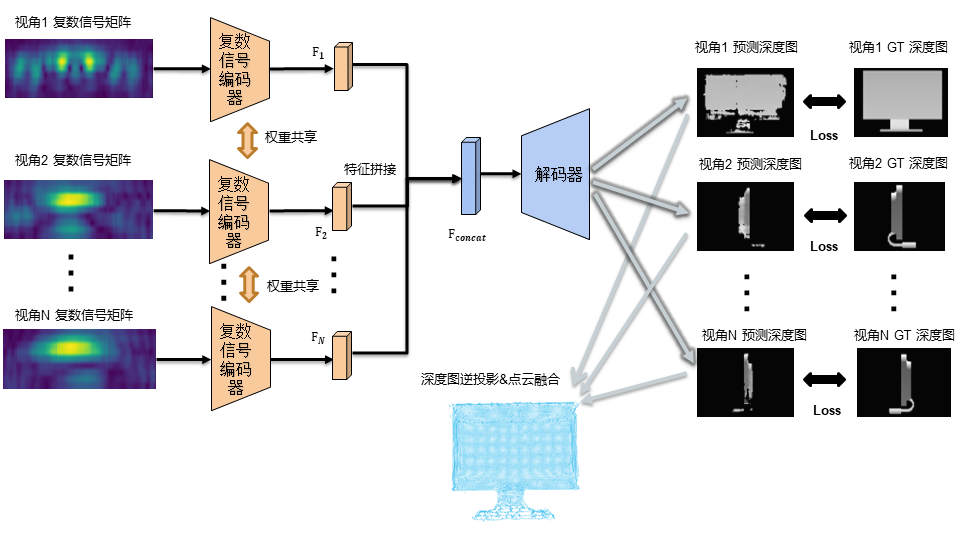
\includegraphics[width=1.0\textwidth]{Figures/网络框图1.png}
    \caption{网络模型框架}
    \label{fig:model1}
\end{figure}

  模型的输入为多个视角下采集到的复数雷达信号矩阵，视角$N$下的复数信号矩阵经过复数信号编码器模块来提取该视角下的物体结构信息对应的隐层特征向量$F_N$，考虑到不同视角下的雷达信号的特征空间是统一的，并且为了避免模型参数量过大产生的过拟合现象，所有视角使用的复数信号编码器模块都是权重共享的。从多个视角下的雷达信号中提取的隐层特征向量会经过特征拼接来获取全局的特征向量$F_{concat}$，之后输送到解码器模块中。在解码器模块的设计上，首先需要考虑的是模型的输出形式，直观上，我们很容易想到让模型直接输出$N\times 3$的张量，对应点云中$N$个点的三维坐标，之前也有工作采取了这样的做法\cite{fan2017point}，然而，由于点云是一堆无序点的集合，即使实际点云相同也可能对应不同的点云排列，模型如何在从隐层特征空间向点云张量映射过程中保持点云排列不变性是一个挑战，虽然现有的倒角距离(Chamfer Distance,CD)损失函数和推土机距离(Earth Mover's Distance,EMD)损失函数在理论上满足排列不变性，但在实际应用过程中仍存在着局限性，例如倒角距离损失函数对异常点敏感，每个点只考虑了最近的邻居，容易忽略整体结构；推土机距离损失函数的计算时间复杂度过高，当点云中点数较多时计算代价过高。另外，使用上述损失函数直接对点云坐标进行回归优化，会导致网络难以捕捉复杂的几何结构，忽略了空间连续性，生成的点云可能会出现不均匀分布或离群点，影响重建质量，因此，本文考虑让网络模型输出多个视角下的深度图，这些视角的相机参数在采集深度图Ground Truth时已经确定，在模型训练阶段，我们对模型输出的深度图进行回归优化，在测试阶段，我们根据每个视角的相机参数来对模型输出的深度图进行逆投影得到局部点云，将多个视角的局部点云对齐到同一坐标系后并进行融合得到最终的全局点云。
\xsubsection{复数信号编码器模块}{Complex Signal Encoder Module}
从雷达复数信号矩阵中提取出物体的三维结构信息是一个极具挑战性的任务，本文提出了一种基于一维卷积的复数信号编码器模块，有效地从复数信号矩阵中提取出了物体三维结构相关的特征向量。

传统的卷积神经网络针对的是实数形式的输入，无法有效处理复数形式的输入，有些工作使用复数卷积神经网络来处理复数输入\cite{8920038,wang2021through,zhang2021cv,mu2021cv}，然而复数卷积神经网络需要重新定义更复杂的正向传播和反向传播等操作，这也导致复数卷积神经网络训练过程中收敛速度极慢难以训练，同时在性能表现上也并未取得明显的优势；与之相对应的另一种做法是通过将复数输入拆分成两路输入，对应复数的实部和虚部，对两路输入分别做处理，之后将特征进行融合，这种做法在对复数信号使用时具有天然的合理性，因为复数信号的实部和虚部有着真实的物理意义，代表着信号的I路和Q路，之前的工作对这种方法的有效性进行了验证\cite{zheng2021more}，相比于复数卷积神经网络，这种做法不破坏原有的卷积神经网络结构，并且具有更好的计算效率和训练稳定性，因此，本文同样采取这种方式。

另一个需要考虑的问题是，模型的输入为$9\times 2800$的信号矩阵，该输入应该被当做是9通道的一维序列使用一维卷积去提取特征，还是当做单通道的$9\times 2800$二维矩阵使用二维卷积去提取特征。回顾信号矩阵的物理意义，9对应的是9个相邻的距离箱，2800对应2800个虚拟天线，两个维度的物理意义不同，与二维图像两个维度上的相邻像素共同构成空间局部特征并不类似，同时信号矩阵在两个维度上的尺度差异过大，难以设计合理的二维卷积核尺寸，因此，针对该信号矩阵，更合理的做法是将其看做是包含9个通道的长度为2800的一维序列，使用一维卷积去提取相关特征。复数信号编码器模块的结构如图\ref{fig:encoder}所示。

\begin{figure}[h]
    \centering
    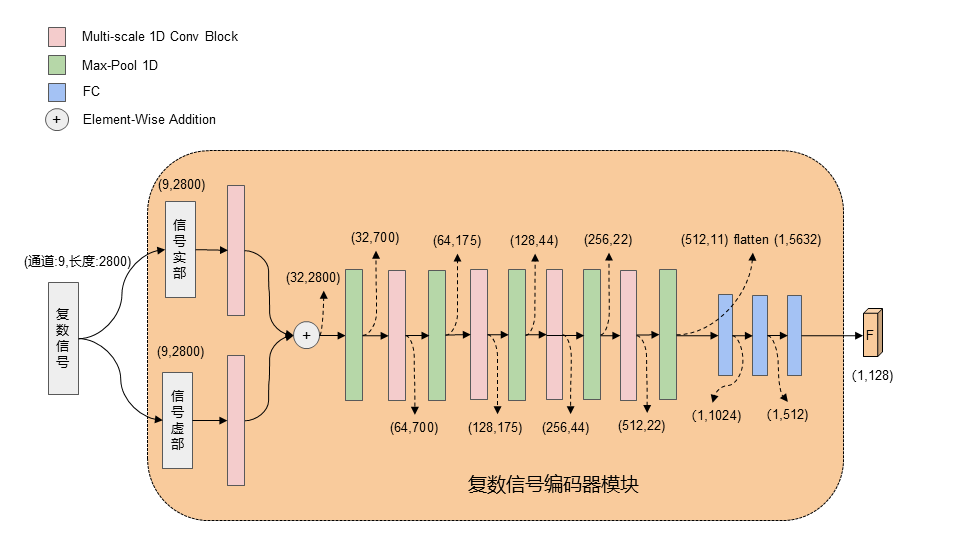
\includegraphics[width=1.0\textwidth]{Figures/encoder.png}
    \caption{复数编码器模块}
    \label{fig:encoder}
\end{figure}

通道数为9，长度为2800的复数信号被输入复数编码器模块后，被拆分成相同尺寸的信号实部和信号虚部，作为两路输入，分别输入到两个多尺度一维卷积块(Multi-scale 1D Conv Block)中，之后使用逐元素相加的方式来将两路多尺度一维卷积块输出的特征进行融合合并为一路，之后使用5级多尺度一维卷积块搭配最大池化(Max-Pool)操作来逐步扩大中间特征图的感受野，特征图长度从2800缩小到11，通道数从32增长至512，通过多级的卷积和池化逐步提取输入信号从局部到全局的特征，最后，将多通道特征图铺平至一维，得到长度为5432的特征向量，并经过三层全连接(Fully Connected,FC)层来对特征向量进行压缩，得到了最终的长度为128的特征向量。其中，多尺度一维卷积块是针对本文信号输入以及中间特征图设计的一个卷积模块，设计过程中参考了波束成形算法中的一些思想。波束成形(Beamforming)算法是雷达系统中常用的一种算法，其目标在于通过调整虚拟天线阵列的相位和幅值权重，使接受信号在特定方向相干叠加，而一维卷积的过程与之类似，模型训练过程中卷积核的可学习参数相当于动态学习虚拟天线阵列中各天线的加权系数。在波束成形算法中，使用不同数量的相邻虚拟天线对应着不同的空间分辨率，在卷积中使用不同的卷积核可以取得类似的效果，小卷积核模拟窄波束，聚焦局部虚拟天线，大卷积核模拟宽波束，覆盖更广天线范围，因此，在多尺度一维卷积块里，使用了3,5,7,9四种尺寸的卷积核，对应不同的空间分辨率，最终将四种卷积核卷积得到的特征图逐元素相加融合输入到激活函数中，为了保证相加时尺寸相同，四种卷积核使用了不同了填充(Padding)尺寸，多尺度一维卷积块的结构如图\ref{fig:multi-scale}所示。

\begin{figure}[h]
    \centering
    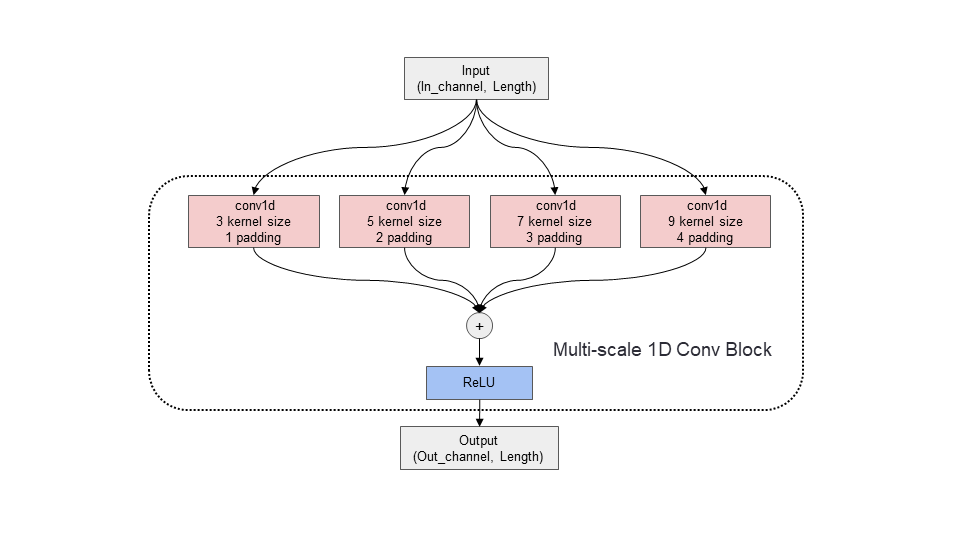
\includegraphics[width=1.0\textwidth]{Figures/multi-scale-conv.png}
    \caption{多尺寸一维卷积块}
    \label{fig:multi-scale}
\end{figure}

\xsubsection{解码器模块}{Decoder Module}
复数信号编码器模块从多视角下的雷达信号中提取到了包含物体三维结构的特征向量，并将多个视角下的特征向量进行拼接得到了融合之后的特征向量$F_{concat}$，解码器模块则负责从作为中间表示的特征向量$F_{concat}$逐步生成目标的多视角下的深度图输出。解码器模块的结构如图\ref{fig:decoder}所示，长度为512的$F_{concat}$特征向量输入到解码器后，首先经过三层全连接层来对拼接后的特征向量进行进一步的融合以及升维，特征向量的长度逐步从512提升到4096。由于我们最终需要得到的是多个视角下的深度图，这是一个典型的二维结构输出，因此在全连接层之后，我们对特征向量进行了重新排列，将其组织成了一个$256\times 4 \times 4$的二维特征图，对应$通道数 \times 高 \times 宽$，在之后的计算过程中，需要对该二维特征图进行逐步的特征提取和上采样，将其尺寸逐渐扩展至目标输出尺寸。对于二维特征图进行特征提取和上采样，最常见的做法是使用反卷积(Transposed Convolution)操作，反卷积操作的核心思想是通过插入零值并应用卷积操作来放大特征图的尺寸，这种操作被广泛应用于语义分割、图像超分辨率和生成对抗网络等任务中，然而，由于反卷积中的插零操作会导致卷积核在覆盖输入时产生不均匀的重叠模式，进而导致反卷积的输出产生棋盘状伪
影。与之相对应的另一种做法是通过插值(Interpolation)+卷积的操作来替代反卷积操作，相比于插零操作，使用插值来实现的上采样更加平滑，避免了卷积核覆盖时的不均匀重叠，消除了反卷积产生了期盼伪影现象，之后再使用标准卷积操作对特征图进行进一步特征提取，多个工作\cite{karras2017progressive,lin2018learning}已经证明了该操作的有效性，因此，本文也使用了这种操作来对特征图进行上采样和特征提取。在解码器模块中，对于$256\times 4 \times 4$的二维特征图，通过五层的双线性插值(Bilinear Interpolation)操作搭配二维卷积操作，将特征图尺寸扩展至$48 \times 128 \times 128$，之后，通过最后一层卷积操作得到$2N \times 128 \times 128$的最终输出，该输出的通道数为2N，N对应的是输出视角个数，前N个通道的输出对应的是N个视角深度图的预测，后N个通道的输出则是N个视角下物体所占据像素的掩膜(Mask)，掩膜的作用在于对物体所处空间位置进行精确预测，排除掉剩余的无用像素点。为了降低模型的学习难度，我们为深度图输出添加深度先验，具体为，将Ground Truth深度图的渲染深度预设为深度值偏置，模型输出的预测深度值是相对于该预设深度的偏移量，因此，模型输出的深度图与预设深度值相加才是最终的深度图预测，通过这种方式，减少了模型预测深度的可能分布空间，有利于模型训练。

\begin{figure}[h]
    \centering
    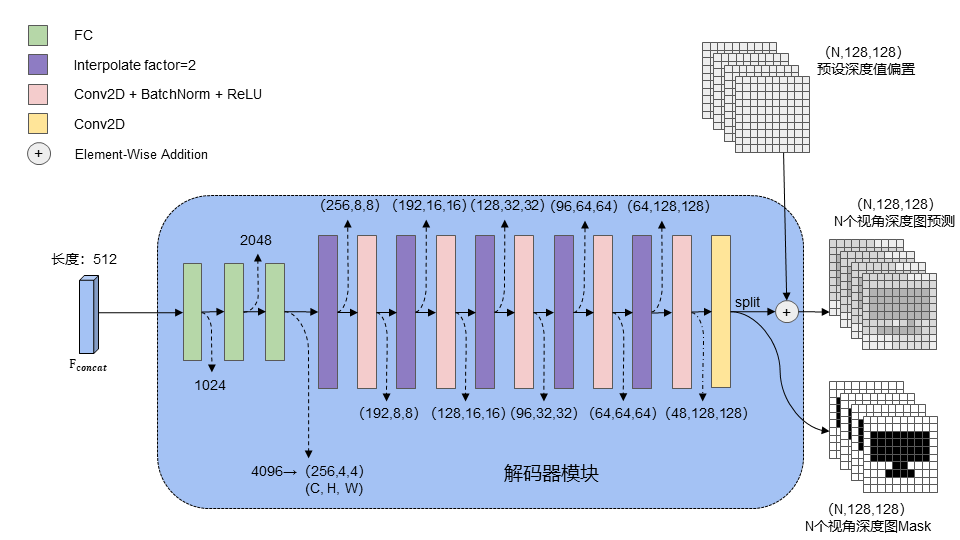
\includegraphics[width=1.0\textwidth]{Figures/decoder.png}
    \caption{解码器模块}
    \label{fig:decoder}
\end{figure}
